%************************************************
\chapter{User Study}\label{ch:userStudy}
%************************************************

The purpose of the music player described in chapter \ref{ch:implementation} is to examine user behaviour regarding the focused-casual continuum. The idea behind this concept is that users can vary their level of engagement for a certain action while not being bound to interact strictly focused or casual with the device. The three interaction techniques introduced in section \ref{sec:UserInterface} and the variable amount of control they offer to the user create different levels in the focused-casual continuum. It is interesting to see whether users recognize and use the different levels of engagement. \\

\section{Procedure}\label{sec:studyProcedure}
However, the viability and beneficing of the system also needs to be confirmed by users in form of a study. Ten participants (2 female, age 21-29 $\overline{x}$=26, $\sigma$=2.47) with different backgrounds were invited. All participants own a smartphone, but only one person owns a smartwatch. Eight participants already had some experience with gesture controlled devices such as the Nintendo Wii or Microsoft's Kinect. Nobody used speech controlled devices beforehand. Before the actual experiment started, the music library and the input techniques were introduced. In a fifteen minute training session the participants were able to acquaint themselves with the music player and practice especially the gesture input. Every participant was then observed while using the music player in six different scenarios that were both private and in public. In each scenario the participants wore the smartwatch on their left wrist and were sometimes more, sometimes less either physically or mentally distracted. The order of the scenarios for each participant was determined using a 6x6 latin square in order to prevent learning effects. \\

Scenarios and their settings\footnote{Bicycle and headphones were provided but one could bring her own to feel more comfortable.}:
\begin{description}
	\item[Office Work]{The participants are seated at a desk in an office. Their task is to copy a text from a sheet of paper to a file on a laptop thus being mentally and physically distracting. This scenario is in a private surrounding.}
	\item[reading on couch]{The participants are seated on a couch in a private living room. Their task is to read a chapter from a book and summarise the content afterwards.}
	\item[Riding a Bicycle]{The participants are riding a bike on a public parking area. Their task is to follow a pre-defined route (depicted in figure \ref{fig:parkingRoute}). The distraction is both mental and physical.}
	\item[joggin]{The participants are jogging the same route on the parking area (depicted in figure \ref{fig:parkingRoute}), thus being in public and physically distracted.}
	\item[Walking mentally distracted]{The participants are walking a pre-defined public route (depicted in figure \ref{fig:walkingRoute}) playing a memory game on a mobile phone. This is mentally distracting. Touch is still possible.}
	\item[Walking physically distracted]{The participants are walking the aforementioned pre-defined public route (depicted in figure \ref{fig:walkingRoute}) carrying a bag in their right hand. This is physically distracting.}
\end{description}

\begin{figure}[bth]
	\myfloatalign
	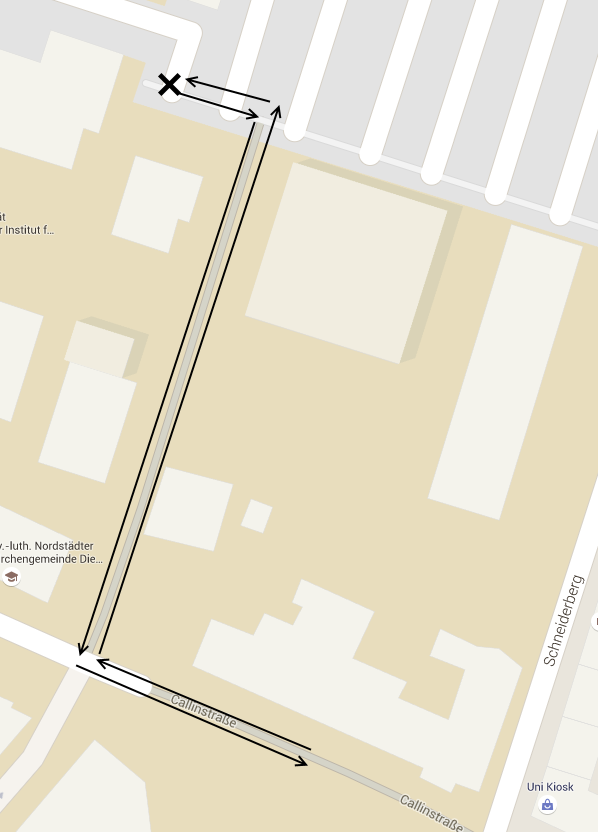
\includegraphics[width=.7\linewidth]{img/walkingRoute.png}
	\caption{Z-shaped route for both of the walking scenarios. During the day this route is much-used by students and other people.}
	\label{fig:walkingRoute}
\end{figure}

\begin{figure}[bth]
	\myfloatalign
	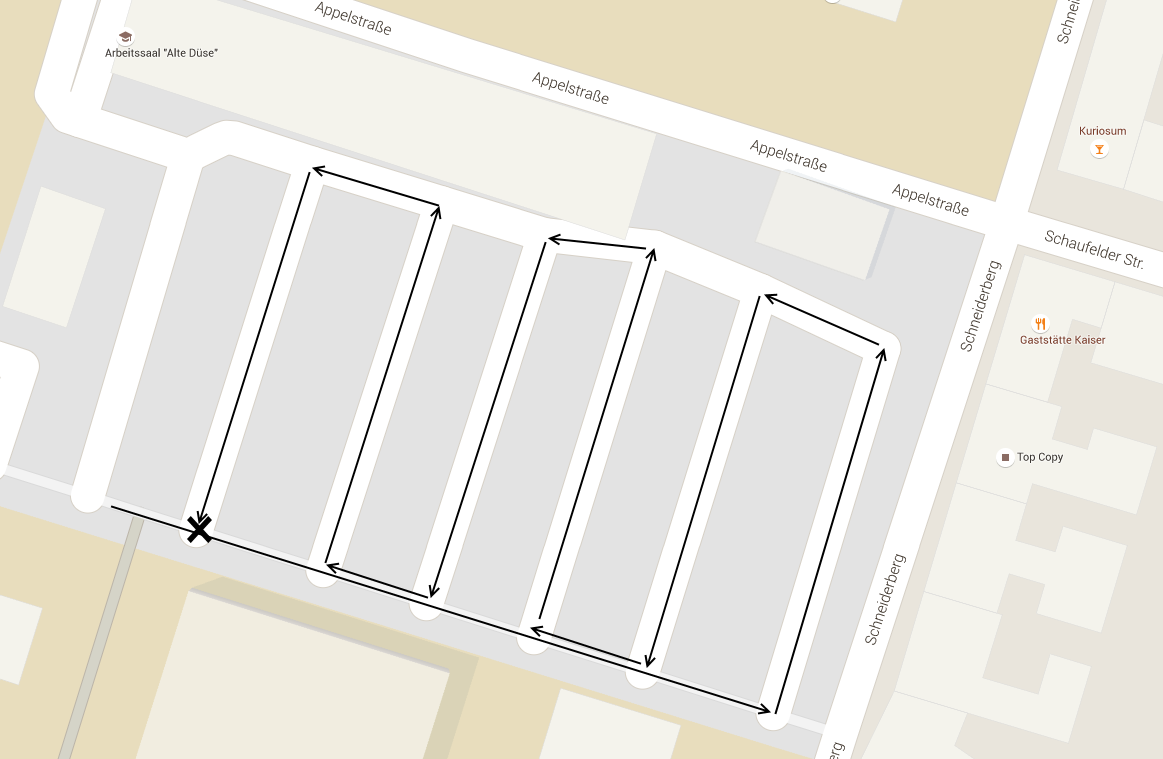
\includegraphics[width=.8\linewidth]{img/parkplatzRoute.png}
	\caption{Zigzag route completely on a parking area for the bicycle and jogging scenario. Participants had to mind arriving and leaving cars and other cyclists.}
	\label{fig:parkingRoute}
\end{figure}

To force the participants to interact with the music player, they were tasked with eight coarsely formulated player interactions in each scenario. For every forced interaction the participant could always freely choose between at least two interaction techniques to use, however, scenario constraints made using some techniques more difficult, e.g. using touch on bicycle. The use of each interaction technique was recorded during the experiment session ignoring interactions with recognition errors. Table \ref{tab:scenarioTasks} lists the interaction tasks and the possible interaction techniques that generally could have been used.

\begin{table}[h]
	\myfloatalign
	\begin{tabularx}{\textwidth}{XX} \toprule
		\tableheadline{Forced Interaction} & \tableheadline{Possible techniques} \\ 
		\midrule
		1. start a playlist & touch, speech \\
		2. adjust the volume & touch, speech, gesture \\
		3. toggle shuffle & touch, speech \\
		4. skip one or more songs & touch, speech, gesture \\
		5. change song relative to a chosen audio feature & touch, speech \\
		6. skip one or more songs & touch, speech, gesture \\
		7. play song from different genre & touch, speech \\
		8. pause current song & touch, speech, gesture \\
		\bottomrule
	\end{tabularx}
	\caption{Interaction tasks for each scenario instructed in this specific order. The skip to next song task was instructed twice in each scenario.}
	\label{tab:scenarioTasks}
\end{table}

\section{Results}\label{sec:studyResults}
In addition to the experiment every participant answered a questionnaire about the experiences they made. First, they were asked to classify their music listening behaviour on a scale from 1 to 5 where 1 means they choose every song they listen to by themselves and 5 means they turn the music on in the morning and turn it off again in the evening. Figure \ref{fig:listenerTypes} shows the distribution of listener types that participated in the experiment. Most people rated themselves to be a mixture of both extreme listening types. This implies that the participants generally interact a lot with a music player.

The answers to the general questions about the experiment (seen in figure \ref{fig:scenarioQuestions}) show an overall agreement on the suitability of the scenarios. 9 out of 10 participants found these or similar scenarios in their everyday life and all participants are regularly listening to music in these situations. Also 9 participants perceived controlling the music player with a smartwatch in contrast to a mobile phone in the scenario contexts as helpful. In General 8 out of 10 participants support the idea of smartwatch aided systems. These answers confirm that a smartwatch in general can be a well suited device for supporting casual interaction.

\begin{figure}[h]
	\myfloatalign
	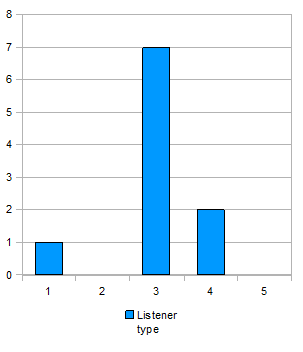
\includegraphics[width=.5\linewidth]{img/listenerTypesPlot.png}
	\caption{Distribution of music listener types. \newline 1 = I choose every song; \newline 5 = I don't care about which song is playing.}
	\label{fig:listenerTypes}
\end{figure}

\begin{figure}[h]
	\myfloatalign
	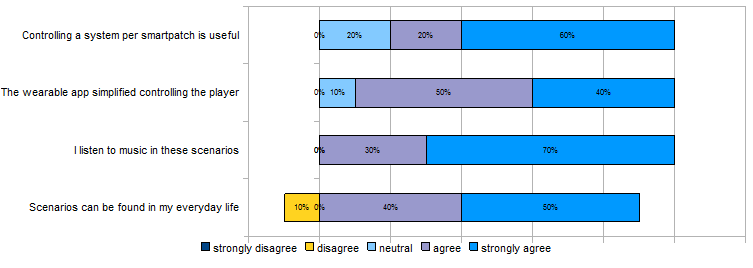
\includegraphics[width=1\linewidth]{img/generalQuestionsPlot.png}
	\caption{General questions about the scenarios and smartwatch controlled systems. Answers were made on a five point Likert scale from strongly disagree to strongly agree.}
	\label{fig:scenarioQuestions}
\end{figure}

\newpage

A big factor for suitability are the offered input techniques and their implementation, though. 
Hence, the participants were asked to prioritize the three input techniques separately for every scenario and every interaction task they were given. 
Values range from 1 (highest priority) to 3 (lowest priority). 
Since some techniques were not possible to use in certain scenarios or for certain tasks, they were automatically prioritized as the lowest. 
Figure \ref{fig:priorityRating} plots the respective results. 
It is striking that gesture input was least prioritized for each task and also for most scenarios, except where touch was not very suitable (e.g. the bicycle scenario). 
Overall the speech input technique was prioritzed the most which is approved by the overall input technique choice during the experiment seen in figure \ref{fig:overallUsage}. 
Figure \ref{fig:inputUsage} additionally plots the amount of input choices that were used most in every scenario and for every task. 
In the bicycle scenario for example eight participants used the speech input for most of the tasks. 
However, gestures could only be used for half of the tasks in contrast to touch and speech input. 
Nonetheless, gestures were, next to speech input, the most chosen technique in the \textit{walking while mentally distracted} scenario. 
In general gestures were avoided where the participant was physically distracted. 
Touch input on the other hand was higher prioritized when the time to complete the interaction did not matter as in the \textit{office work} and \textit{reading on couch} scenario. 
The low usage of speech input for the pause task seen in figure \ref{fig:taskUsage} stands out, though, and was caused by the participants finishing their scenario task before pausing the music. 
Thus, they were able to choose the input technique without physical or mental constrains. 
The averaged rating of the overall control over the music player with each input technique shown in figure \ref{fig:perceivedControl} can be one reason for these usage numbers. 
A high rating would mean that the participant felt to have sufficient control while using the interaction technique. 
Gesture input, however, received a low rating of 3.7 out of 10 mainly caused by falsely recognized gestures which led to unwanted music player actions.

\begin{figure}[h]
	\myfloatalign
	\subfloat[Averaged priority rating for the input techniques in every scenario]
	{\label{fig:priorityScenarios}
	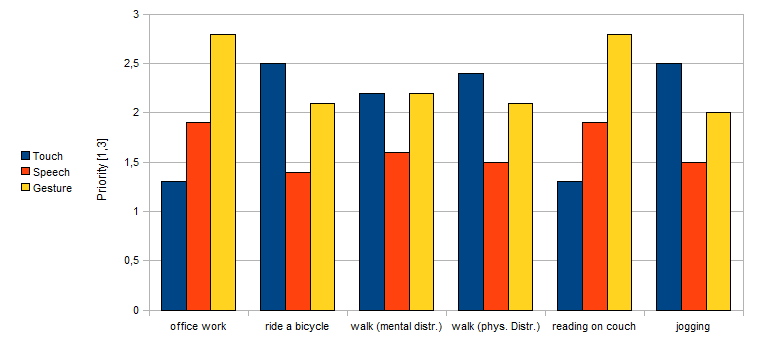
\includegraphics[width=.95\linewidth]{img/priorityScenarios.png}} \\
	\subfloat[Averaged priority rating for the input techniques for every task]
	{\label{fig:priorityTasks}
	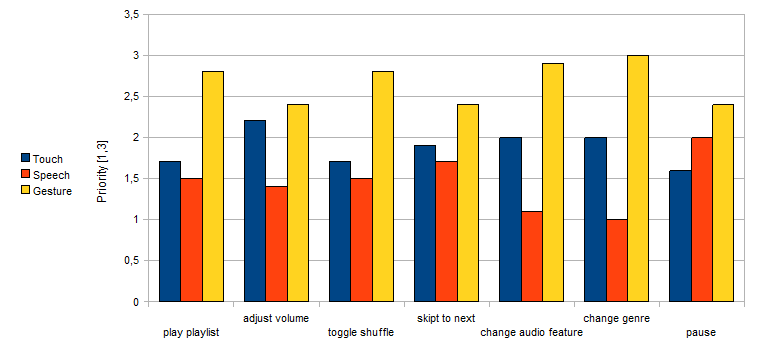
\includegraphics[width=.95\linewidth]{img/priorityTasks.png}}
	\caption{The participants prioritized the three input techniques from 1 (highest priority) to 3 (lowest priority). The values are averaged over all participants.}
	\label{fig:priorityRating}
\end{figure}

\begin{figure}[h]
	\myfloatalign
	\subfloat[Amount of most made choices for each scenario.]
	{\label{fig:scenarioUsage}
	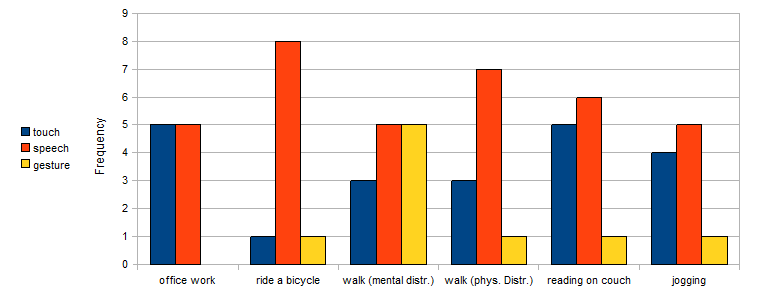
\includegraphics[width=.95\linewidth]{img/scenarioUsage.png}} \\
	\subfloat[Amount of most made choices for each task.]
	{\label{fig:taskUsage}
	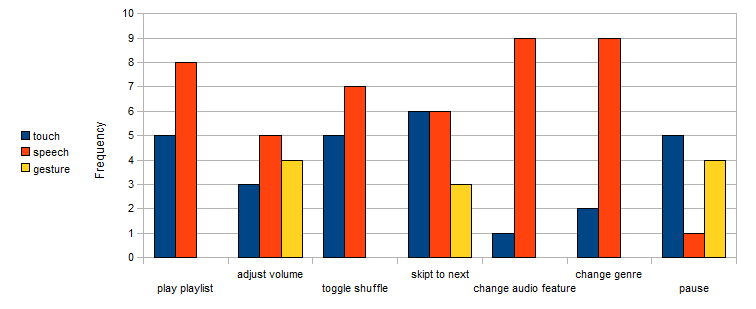
\includegraphics[width=.95\linewidth]{img/taskUsage.png}}
	\caption{Plot of how often an input technique was the most used during a scenario or a task respectivley. Speech input clearly dominates in the bicycle scenario and the complex music player tasks.}
	\label{fig:inputUsage}
\end{figure}

\begin{figure}[h]
	\myfloatalign
	\subfloat[Averaged perceived amount of control over the music player with an input technique while using it. Values range from 0 (no control) to 10 (full control).]
	{\label{fig:perceivedControl}
	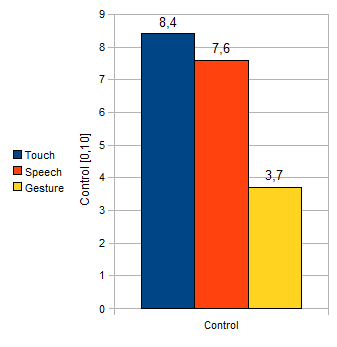
\includegraphics[width=.4\linewidth]{img/perceivedControl.png}} \quad
	\subfloat[Overall usage numbers of each input technique for all participants.]
	{\label{fig:overallUsage}
	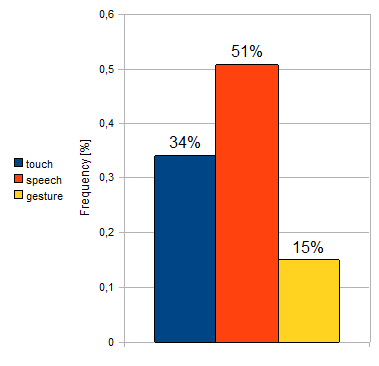
\includegraphics[width=.4\linewidth]{img/overallUsage.png}}
	\caption{}
	\label{fig:controlAndUsage}
\end{figure}

\begin{figure}[h]
	\myfloatalign
	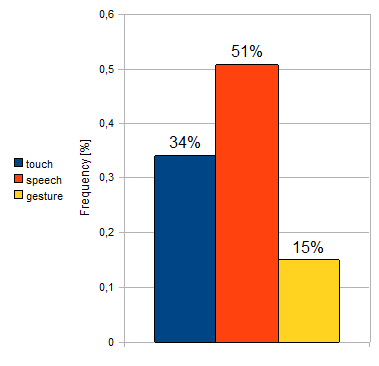
\includegraphics[width=.6\linewidth]{img/overallUsage.png}
	\caption{Overall usage numbers of each input technique for all participants.}
	\label{fig:overallUsage}
\end{figure}

\newpage

Further, the participants were asked to rate the amount of physical or time-wise effort (figure \ref{fig:requiredPhysicalEffort}) and the amount of required attention (figure \ref{fig:requiredAttention}) for each input technique regarding each scenario. Values range from 0 (almost no effort/attention) to 10 (high effort/attention such that current task has to be interrupted). It again stands out that speech input was rated as the best in each scenario. Gestures were often times rated better than touch input, though, but since speech input was apparently much more convenient, gestures were still not used more often.

\begin{figure}[h]
	\myfloatalign
	\subfloat[Required amount of physical effort in each scenario.]
	{\label{fig:requiredPhysicalEffort}
	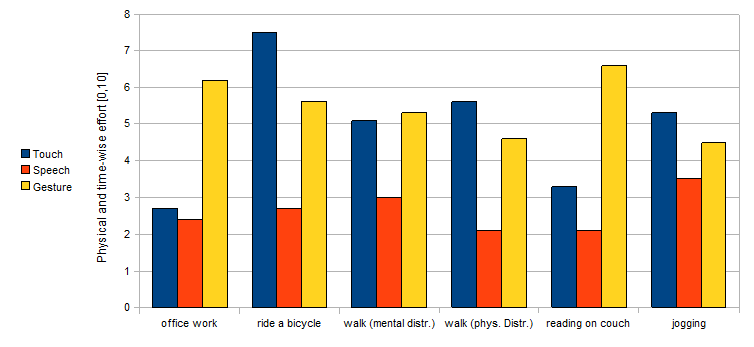
\includegraphics[width=1\linewidth]{img/requiredPhysicalEffort.png}} \\
	\subfloat[Required amount of attention in each scenario.]
	{\label{fig:requiredAttention}
	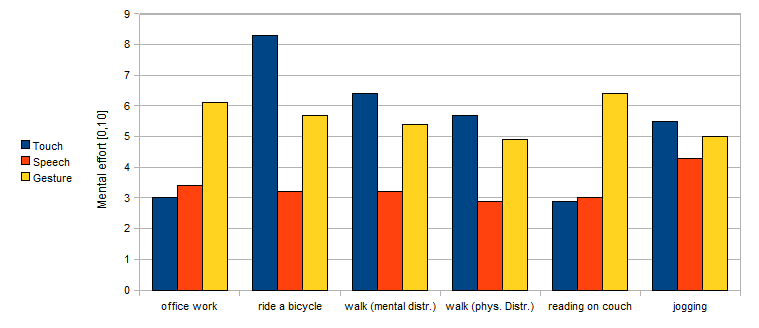
\includegraphics[width=1\linewidth]{img/requiredAttention.png}}
	\caption{Participant rating of required ressources namely physical or time-wise effort and attention for each input technique. Values range from 0 (almost none needed) to 10 (current task has to be interrupted).}
	\label{fig:requiredRessources}
\end{figure}

In order to better understand the input technique choices, the participants were asked to reflect about their usage decisions. \textit{Why did you prefer technique X the most and why did you avoid using technique Y?} Seven participants used the speech input the most and agreed on their arguments for that. It was a novel technique, but at the same time they perceived the technique as powerful, fast, intuitive and not very distracting, so that they could always focus on the current task. Nevertheless, one participant used speech input the least and states a high error rate in noisy situations for the speech recognition as a reason. This participant, together with two others, instead prefered using touch the most and explained it with familiarity and a high success rate. It was also described as fast and accessible for simple commands since the smartwatch was attached to the wrist. On the other hand, touch was also described as highly distracting and slow when used for complex commands like changing the genre or selecting a playlist. Gestures were described as error-prone, time consuming and inconvenient. Concentrating on the beginning of the gesture recording window was claimed to be difficult and distracting. Only one participant had concerns about performing gestures in public describing them as ``looking silly''. None of the other participants was concerned about using speech or gesture input in public. \\

\newpage

Summing up, the results show that a smartwatch is indeed a suited device for supporting casual interaction whether it is used in smart homes or other environments. The three input techniques introduced with the smartwatch already cover a wide area of the focused-casual continuum offering at least one alternative technique, but it depends on the user's context which technique is applicable. Touch input was the prefered technique for all engagement levels when the user's hand or fingers were not occupied. It was, however, only used for complex tasks when the required input time did not matter.
Gesture input was only designed for the simple music player tasks, hence it was expected to not being used often. But gestures were not used very much at all which is related to false recognitions causing a lack of control over the music player. Also speech input was possible to use in every scenario and for each task, thus the participants got quickly used to this technique not considering using gestures instead. It is noteable, though, that the error rate of speech input increases with louder background noises and presumably the technique would then become less appealing to use. Apart from that, the speech input technique turned out to be the most convenient and flexible interaction technique for casual interaction with a smartwatch.


% explain use of wiigee with requirement for simple gestures



%Chapter \ref{ch:relatedwork} 


%*****************************************
%*****************************************
%*****************************************
%*****************************************
%*****************************************




